\chapter{Implementation}\label{imp}
Due to the agile nature of the prototype development, the implementation stage begun while the design phase was still underway. This chapter describes what went into the implementation of the final prototype.

\section{Micro controllers}%Daniel
	Initially during the implementation phase, research went into what kind of micro controller, should be used to construct a working prototype. Initially the Arduino Mega 2560\footnote{Arduino introduction: \url{https://www.arduino.cc/en/Guide/Introduction}} was chosen, but going into the production phase, it became apparent that an external sound source was needed. The Beaglebone Black\footnote{Beagle Bone: \url{https://beagleboard.org/black}} with the Bela shield suited this purpose.
	\subsection{Arduino}%Daniel
		The Arduino devices are a small, but versatile group of micro controllers, used around the world for Do-it-yourself(DIY) projects\footnote{Arduino introduction: \url{https://www.arduino.cc/en/Guide/Introduction}}, that are both easy to use and cheap to obtain. The Arduino Mega, with the ATMEGA2560 chip is one of the more powerful variants, with a bigger EEPROM and more pins than the more commonly seen Arduino Uno. The pin amount was paramount in the decision to which micro controller was needed to control the physical interface, as the design called for a 4x5 grid of fields that should be individually activated. A Piezo buzzer can be connected to the Arduino and be used as both input and output of vibrations. Therefore, it can produce tones by vibrating at different frequencies. However, it is not very loud, and as such will not suffice for producing loud sounds.
		
	\subsection{Bela}%Jens\
		Due to the sound related limitations from the Arduino Mega, since a Piezo Buzzer did not make sufficient noise, it was decided to add a connection to a Beaglebone with a Bela shield\footnote{Bela website: \url{https://bela.io/}}. The Bela provides a broad span of audio processing capabilites to create and manipulate audio as it is compatible with Pure Data(PD). PD is a visual programming language for multimedia that can also be used to create sounds.
	
\section{Code}
	When designing the system for the mat, it came down to three requirements:
	\begin{itemize}
		\item[-] It should be able to save the activated fields in each of the four beats.
		\item[-] It should be able to save the sequences of fields in four separate segments.
		\item[-] It should be able to play back the previously saved segments.
	\end{itemize}
	\subsection{C/C++}%Daniel
		To categorize the data and prepare it for saving on the Mega, two separate structures were made. These structures, as seen in listing \autoref{listing:structs} are called \mintinline{cpp}{SequenceField} and \mintinline{cpp}{Segment}. SequenceField contains an \mintinline{cpp}{int} that holds the octave of the sequence, and a \mintinline{cpp}{Field} array to hold the activated fields.
		
	
		The \mintinline{cpp}{Segment} structure holds a \mintinline{cpp}{SequenceField} array to contain the 4 beats, a \mintinline{cpp}{bool} to keep track of what segment is enabled, and the corresponding LED pin.
		
		\begin{listing}[H]
			\caption{The structs used to contain our data for the segments and their fields.}
			\label{listing:structs}
			\begin{minted}[frame=lines,framesep=2mm,baselinestretch=1.1,fontsize=\footnotesize,linenos]{cpp}
struct SequenceField {
  int octave = 4;
  Field activatedFields[5];
};

struct Segment {
  bool enabled = true;
  int ledPin;
  SequenceField sequence[4];
};
			\end{minted}
		\end{listing}
		\noindent
		To save the segments and their data to persist through restarts, the onboard EEPROM was used. The EEPROM on the Arduino Mega can hold 4096 bytes of data, the segments only take up 611 bytes of that space. Writing the segments into the EEPROM is accomplished by iterating over the \mintinline{cpp}{Segment} array, and put onto the EEPROM according to the size of the structure, as seen in \autoref{listing:writeSegment}.
		\begin{listing}[H]
			\caption{Writing our segment data to the EEPROM}
			\label{listing:writeSegment}
			\begin{minted}[frame=lines,framesep=2mm,baselinestretch=1.1,fontsize=\footnotesize,linenos]{cpp}
void writeSegments() {
  for(int i = 0; i < amountOfSegments; i++) {
	EEPROM.put(i*sizeof(Segment), segments[i]);
  }
}
			\end{minted}
		\end{listing}
		\noindent
		\autoref{fig:flowchartPlayRecord} explains what happens when either the record or play buttons are pressed. Pressing the play button, goes through the enabled segments, and plays the sequences in each. Pressing the record button however starts a more complex routine, starting with going through each field in the current beat and checking if it is activated. Then an empty Field object is made for each field, to record silence in the fields where no user were standing. If a field was activated, then it saves the octave in the sequence and the field in \mintinline{cpp}{activatedFields[]}. In the end it plays the activated fields' sounds.
		\begin{figure}[H]
			\centering
			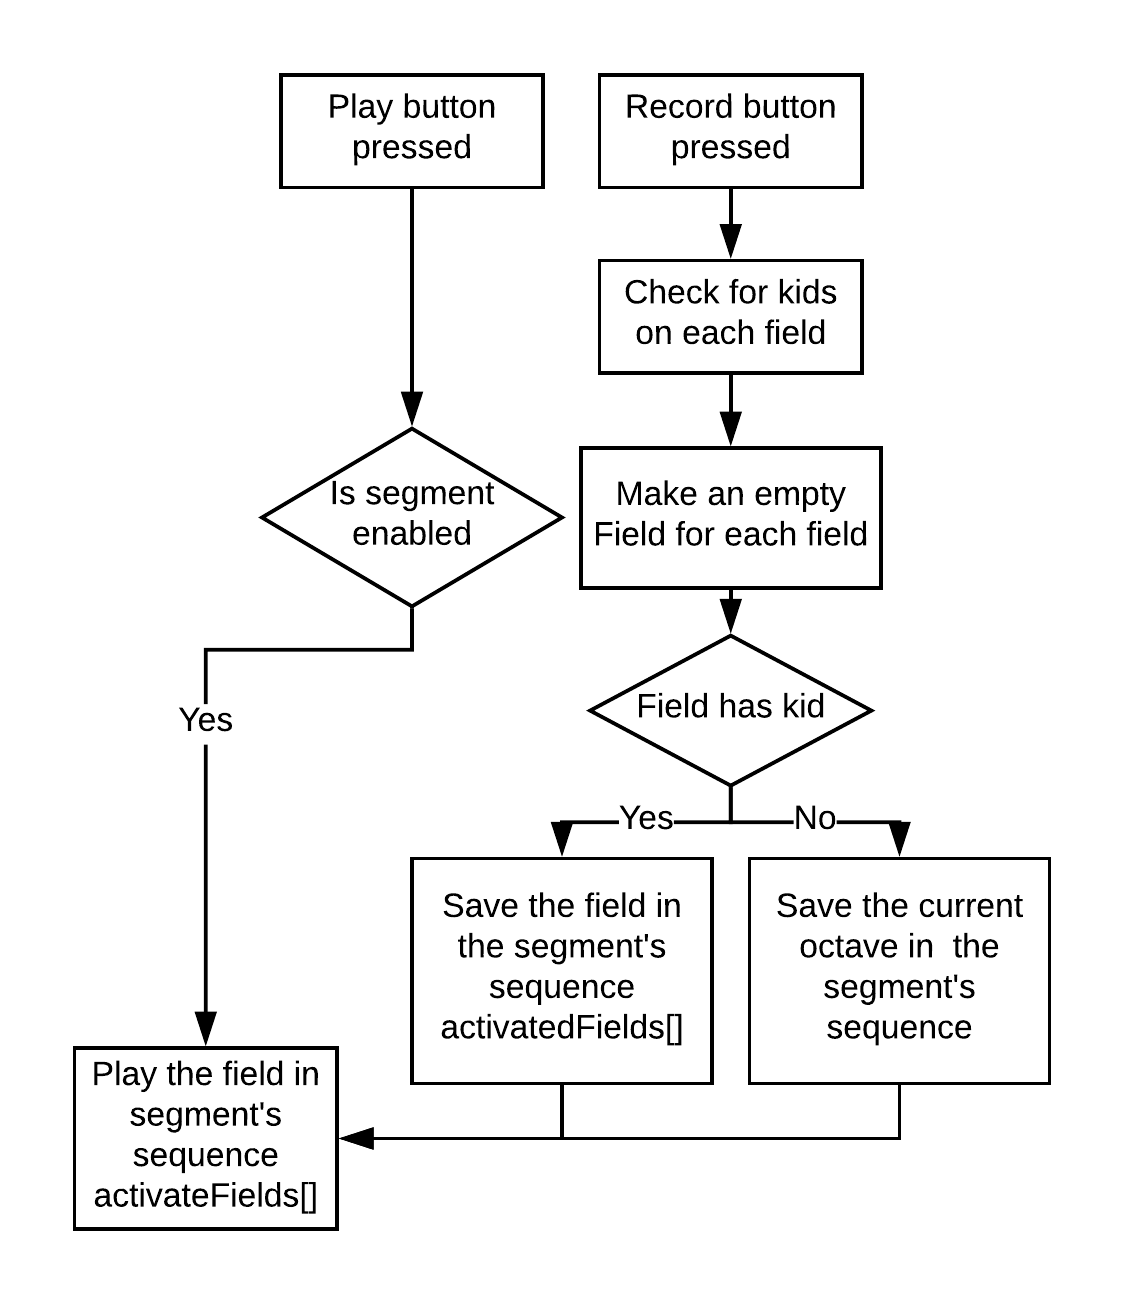
\includegraphics[width=.5\linewidth]{figure/Implementation/flowchartPlayRecord}
			\caption{Flowchart of pressing either the play or record button}
			\label{fig:flowchartPlayRecord}
			\end{figure}
	
		\subsubsection{Libraries}%Daniel
			To achieve all of the functionalities in a short amount of time, two libraries were used in addition to the system,
			the FastLed and Button library. The button library is fairly self explanatory, it is a library with a button class, that makes it easy to read button presses and account for debounce, which eliminates unexpected button presses, that can occur due to mechanical and physical issues. The FastLed library makes it easy to interface with, and control a LED strip or LED matrix.
	\subsection{PureData}%Jens
		\autoref{fig:pdPatch} shows the main patch of the PD code that was uploaded to the Bela. It takes inputs through the Belas' pins from the Arduino Mega. The PD patch is responsible for playing the sounds when the pads are pressed, changing the octave by multiplying or dividing the oscillators' frequencies by two, and playing the count-in sound before recording or playing.
	
	\begin{figure}[H]
		\centering
		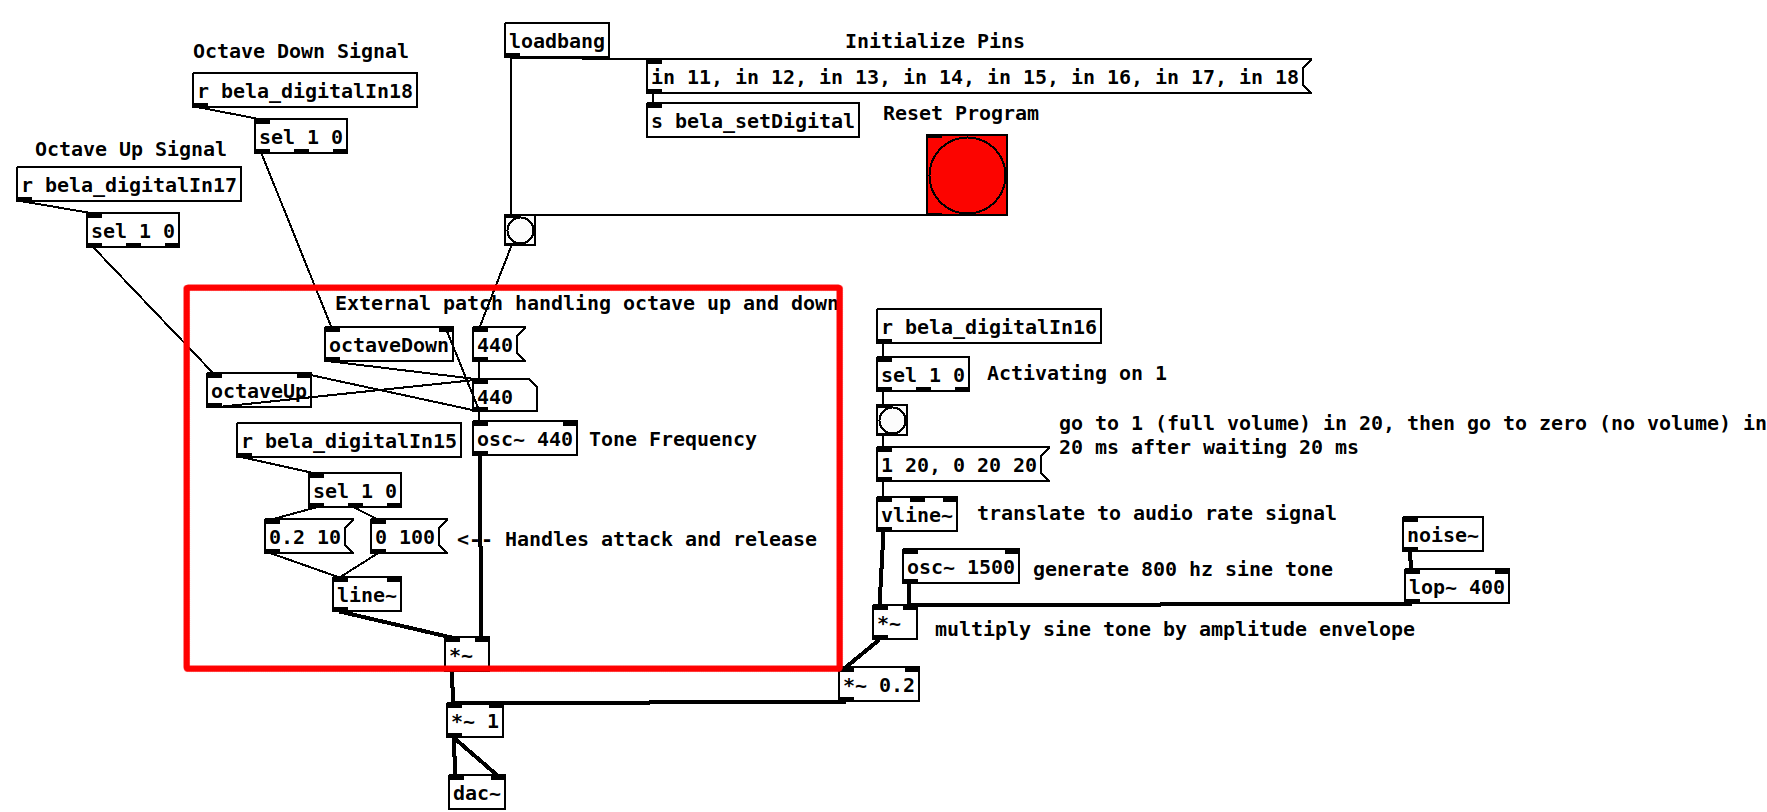
\includegraphics[width=1\linewidth]{figure/Implementation/pdPatch1.png}
		\caption{Figure showing a snippet of the main Pure Data patch for the prototype. The red square is how a tone(A) is handled. This section is repeated throughout the rest of the tones.}
		\label{fig:pdPatch}
	\end{figure}
	To generate sound, the C Major pentatonic scale was used for the five tones. These were generated by an Oscillator object. A functionality for octavating the scale up and down was implemented to add more variety and options. By dividing the current tone frequency by two the octave is lowered and by multiplying by two it is raised. \autoref{tab:toneFreq} the frequencies for the octaves available on the system.
	
	\begin{table}[H]
		\centering
		\caption{Table showing the oscillator tone frequencies for the pentatonic scales in the different octaves.}
		\label{tab:toneFreq}
		\begin{tabular}{|c|c|c|c|c|c|}
			\hline
			Octave/tones & C     & D     & E     & G    & A    \\ \hline
			3            & 130.5 & 146.5 & 164.5 & 196  & 220  \\ \hline
			4            & 261   & 293   & 329   & 392  & 440  \\ \hline
			5            & 522   & 586   & 658   & 784  & 880  \\ \hline
			6            & 1044  & 1172  & 1316  & 1568 & 1760 \\ \hline
		\end{tabular}
	\end{table}
	



\section{The Box}%Jens
In order to conceal wires and micro controllers and to construct an easy way of controlling the various features, a box was created. This section explains how it was built.
	\subsection{CAD}
	    Autodesk's Fusion 360\footnote{Product overview page for Fusion 360: \url{https://www.autodesk.com/products/fusion-360/overview}} with an additional box generation plugin provided a convenient way of creating the blueprint for the control box that would later be used to laser cut the six sides of the box out of a 4mm Medium Density Fiberboard(MDF). Holes were cut into the lid of the box, in order to insert the buttons and LEDs. On the front side facing the mat a square hole was cut that would be used for a custom made plug for easily connecting the mat with the Arduino Mega. For decoration, a G-clef was also cut into the front facing side. On the backside, holes were cut to provide easy access for adding an external speaker through a female 3.5mm jack plug, and also to power the Bela using a USB cable. \autoref{fig:finalbox1} shows how the control box ended up looking.
	
	
	\begin{figure}[H]
		\centering
		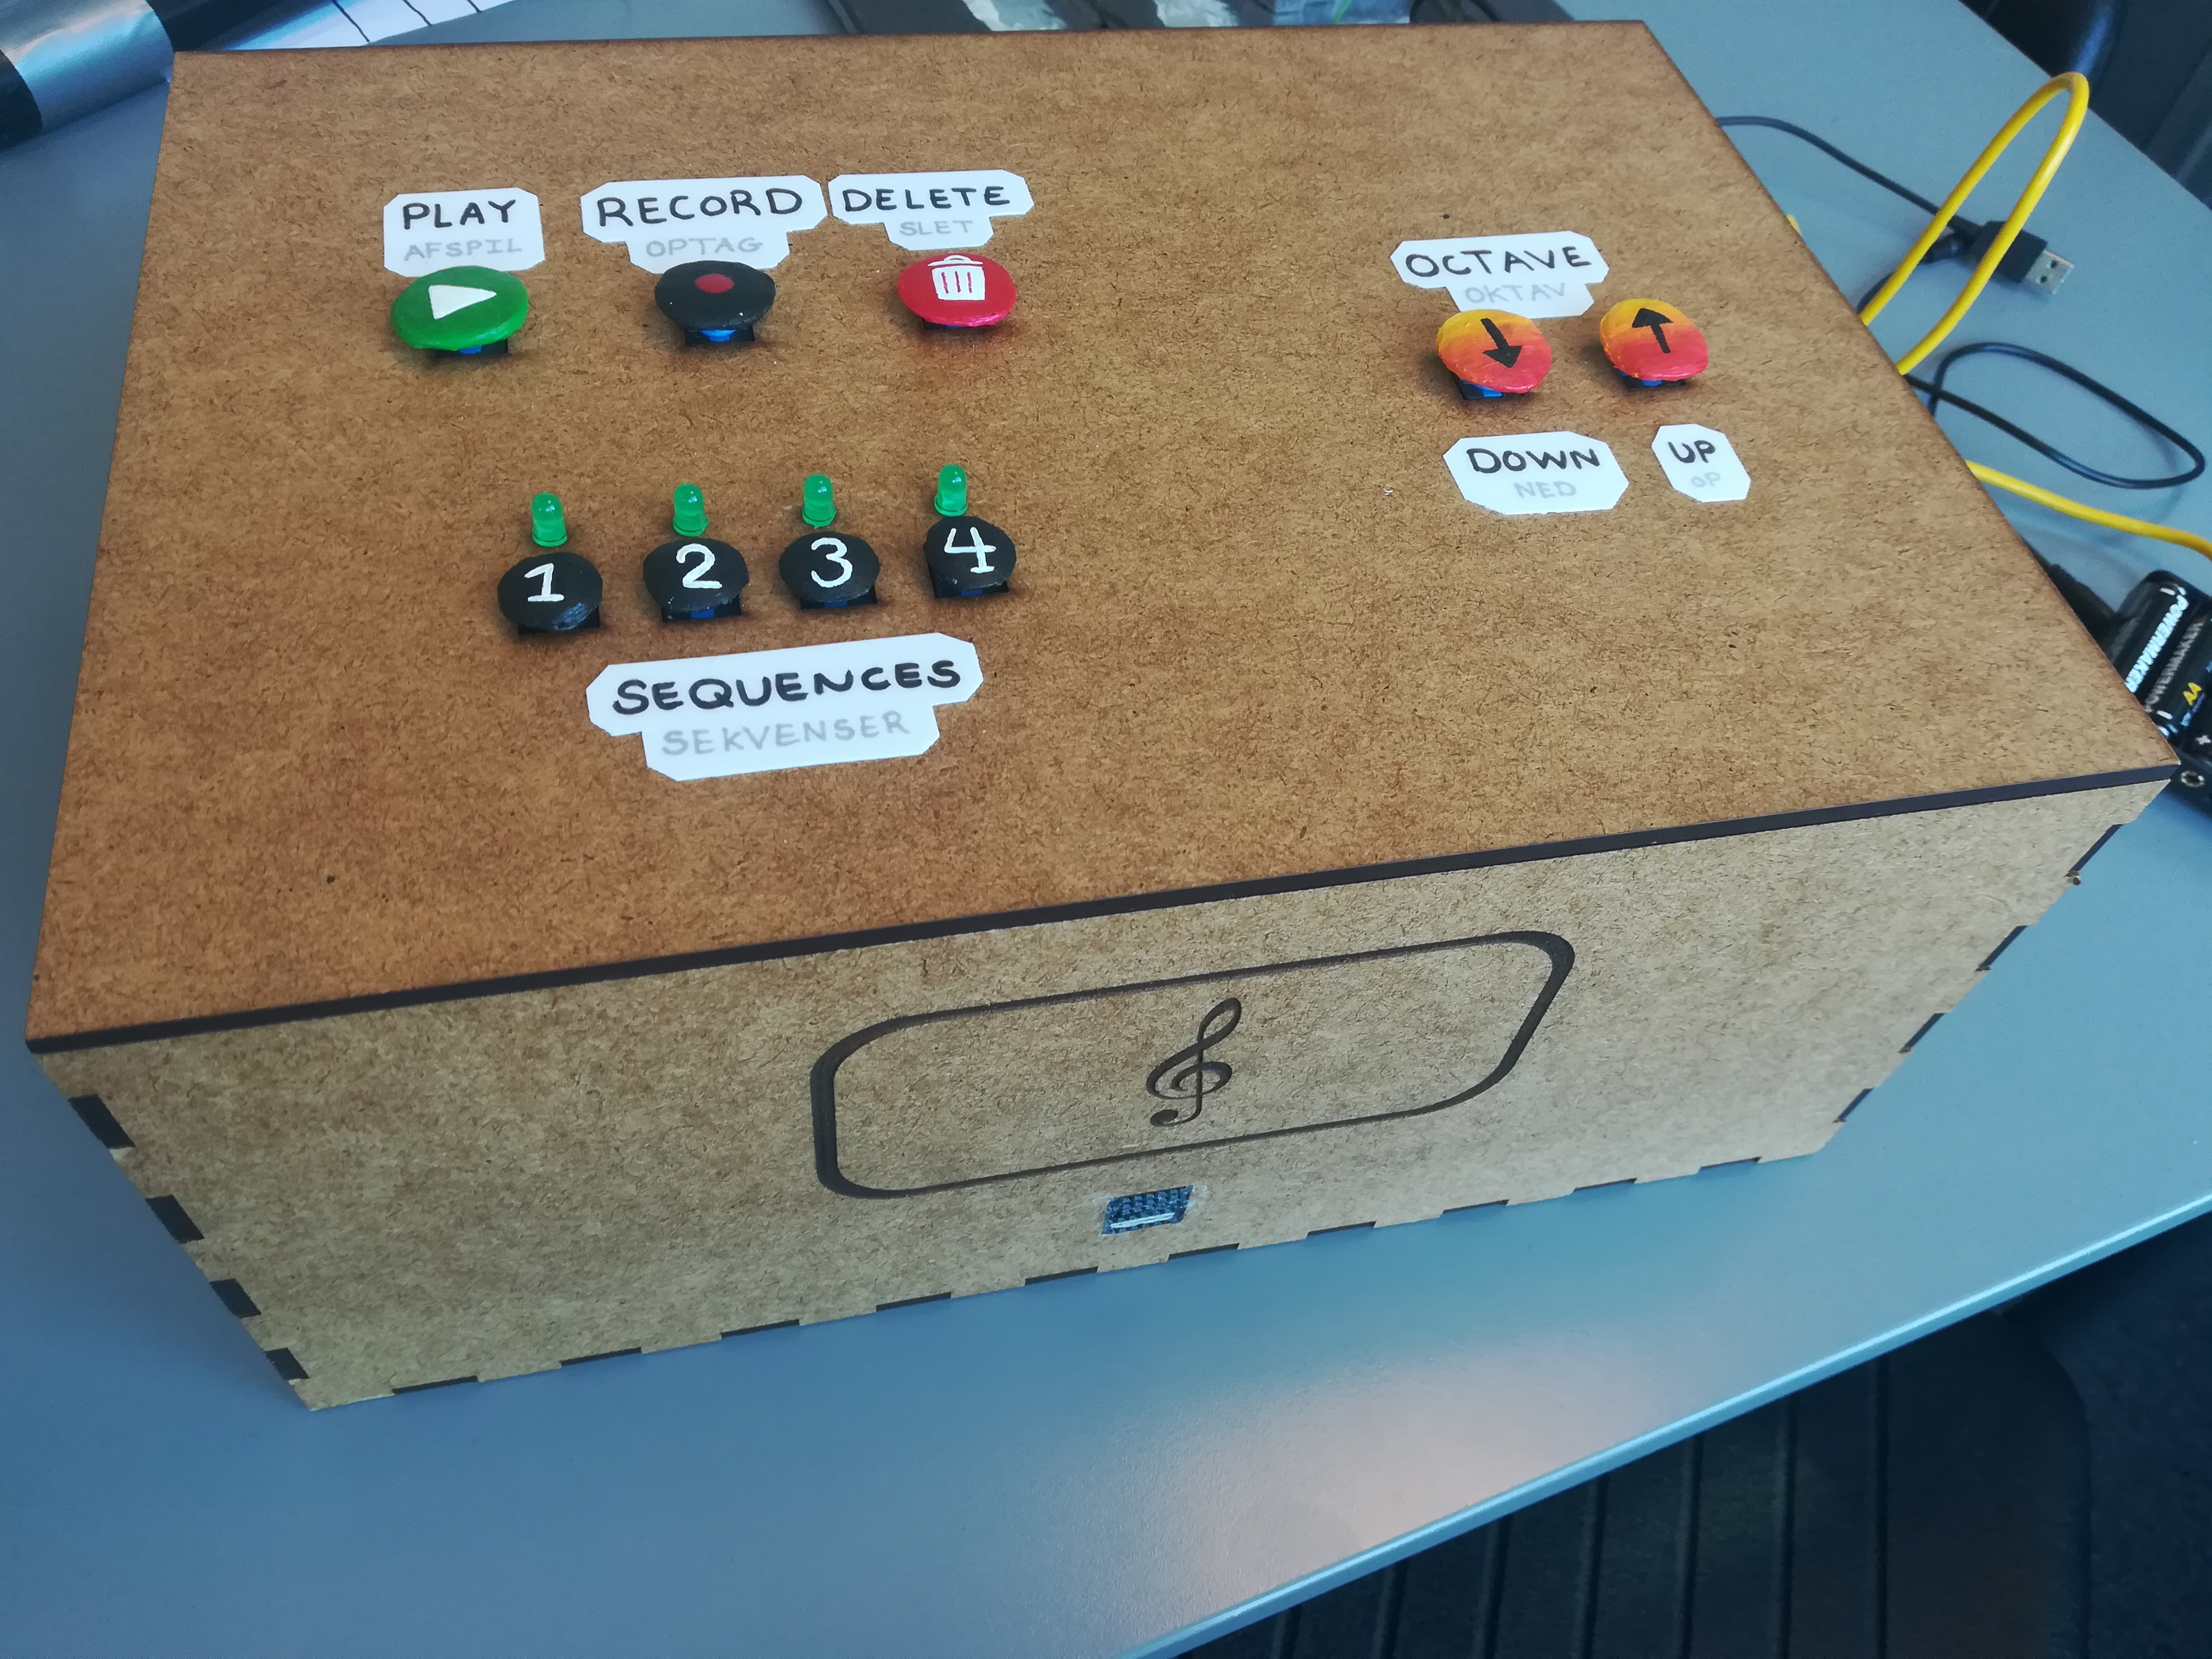
\includegraphics[width=0.9\linewidth]{figure/Implementation/boxFront}
		\caption{Figure showing the final control box after assembly.}
		\label{fig:finalbox1}
	\end{figure}
	
		
	\subsection{Assembly}
	Due to the way the sides of the box were constructed with finger joints that fit together, the box was easy to assemble. With a kerf of 0,275mm, the sides were able to stick to each other without using glue or nails. The custom female mat plug was glued to the inside of the box. This was also the case for the buttons and the LEDs on the lid. These also required wires that were soldered on with extra length, which made it possible to lift the lid of the box without wires being detached from the micro controllers. A rim was glued onto the lid, to hold it in place since the lid was not made with joints (See \autoref{fig:finalbox2}).
	
	\begin{figure}[H]
		\centering
		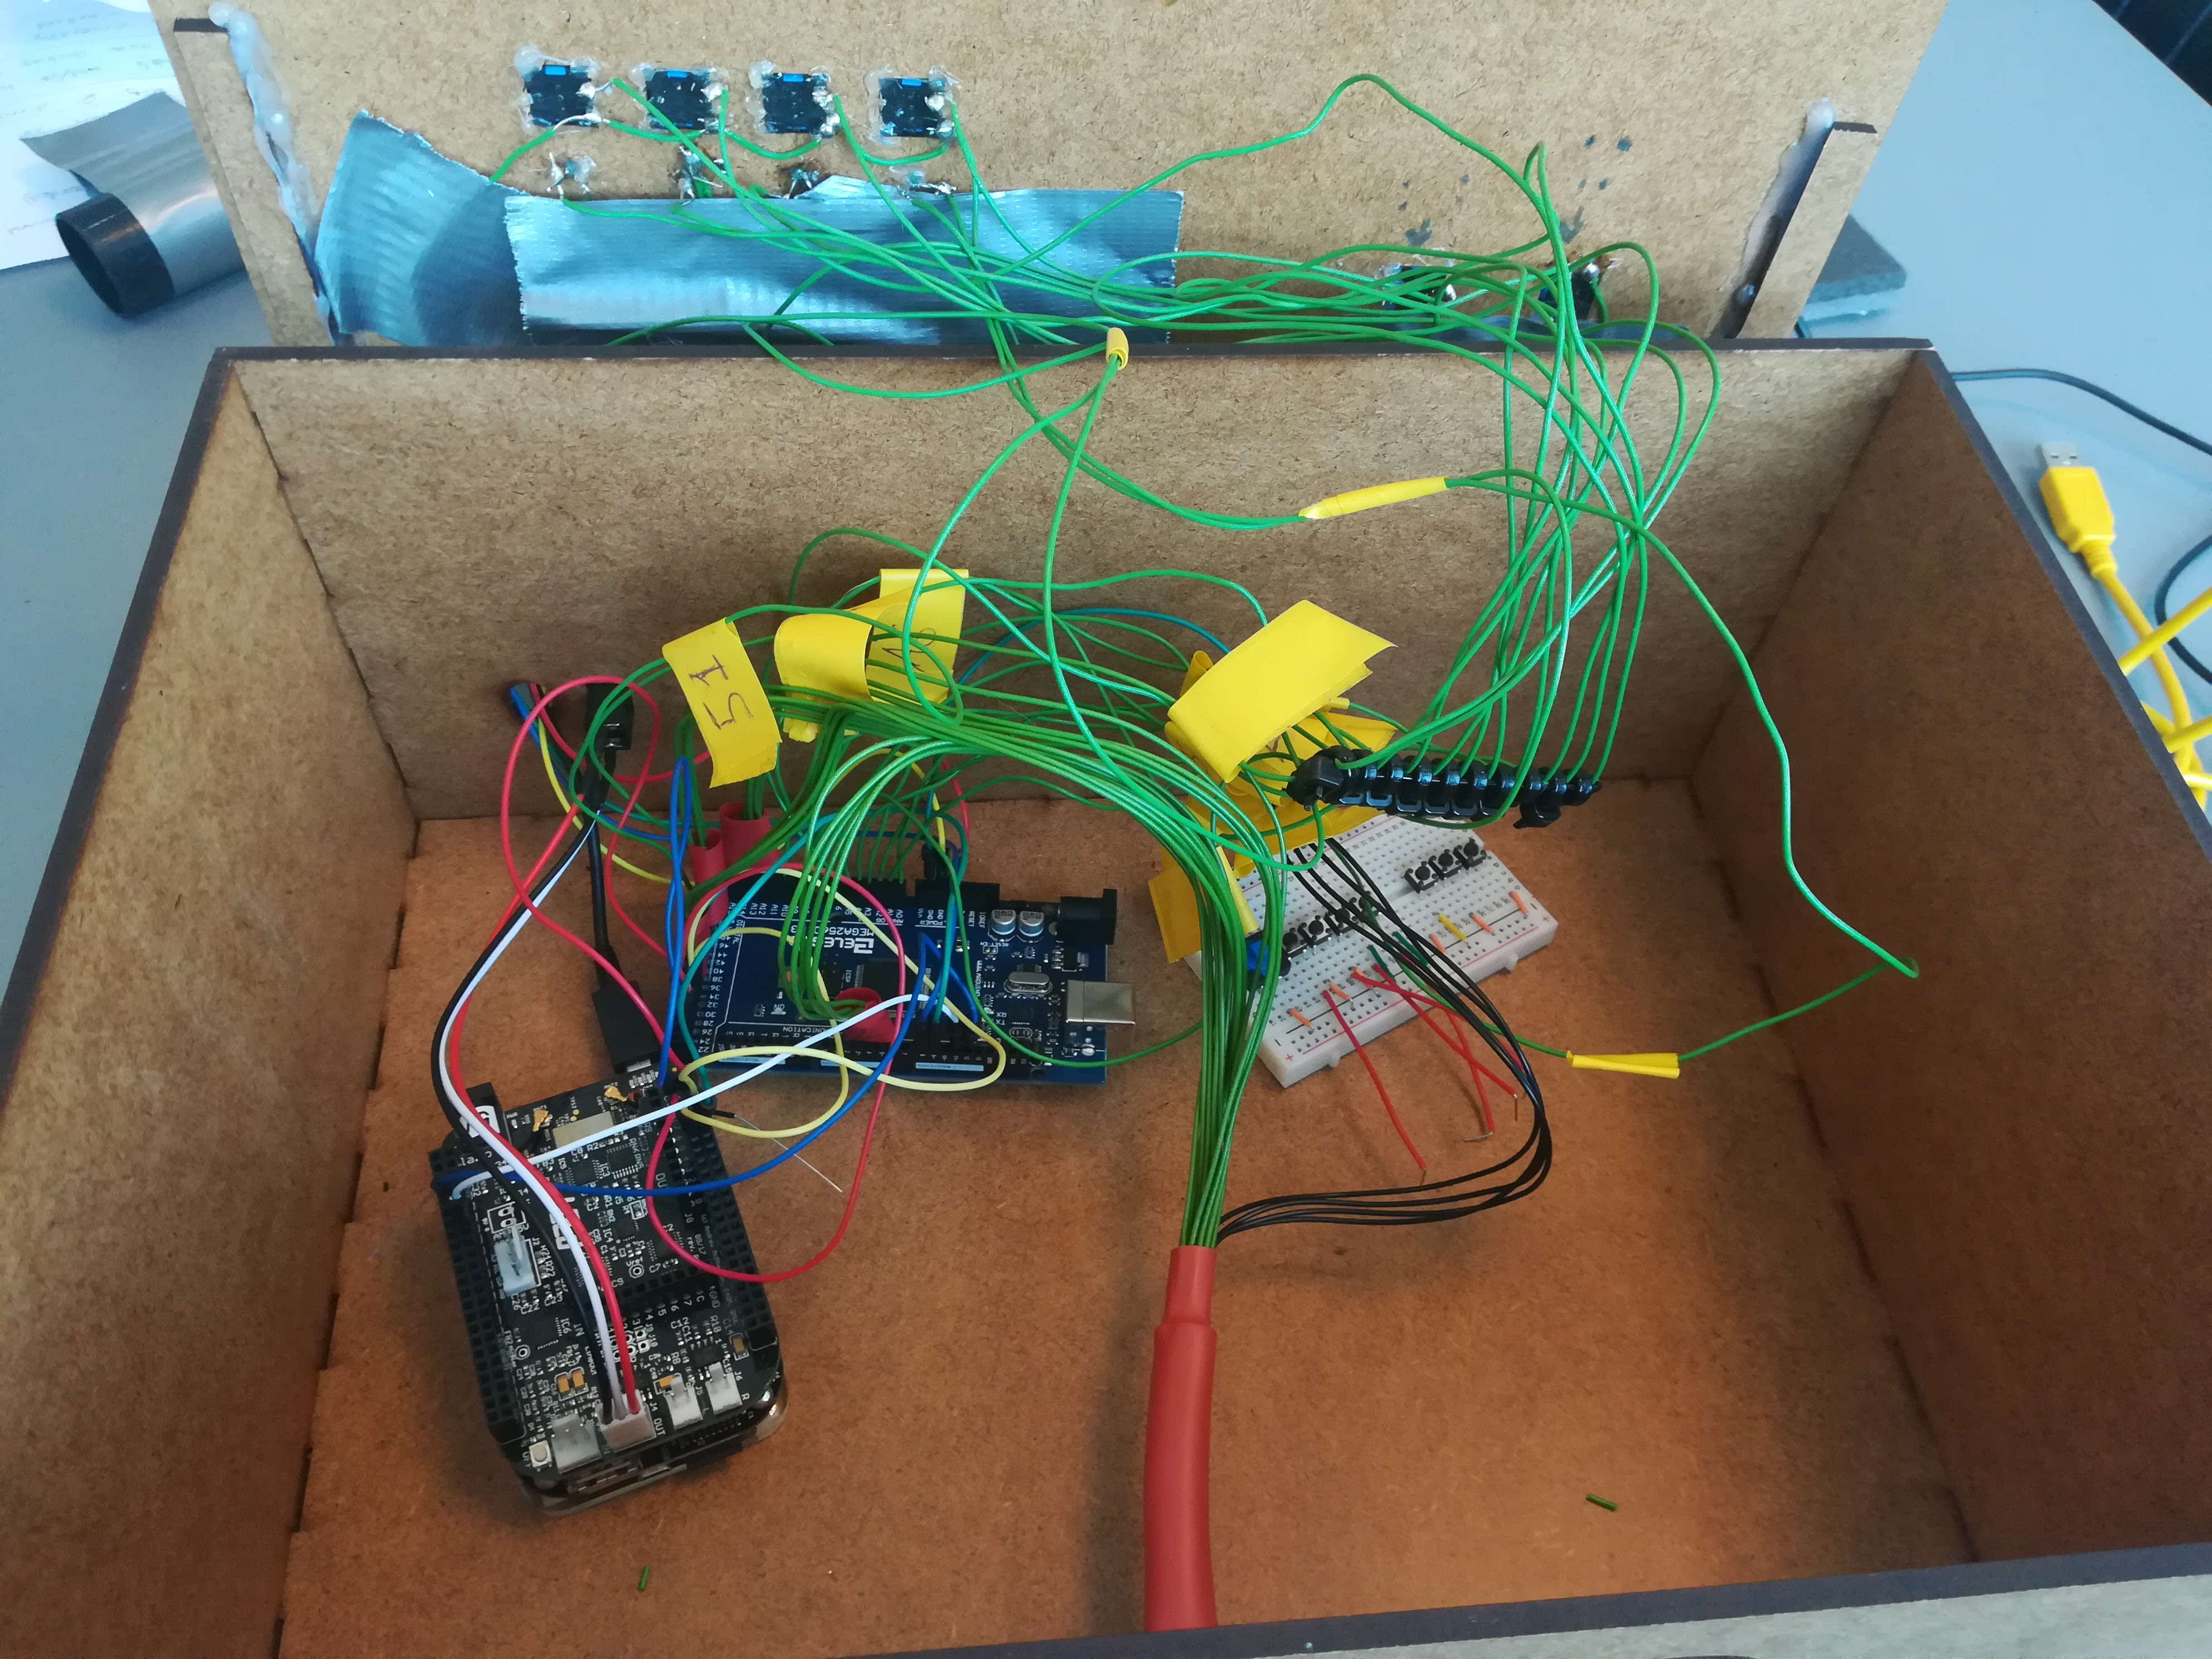
\includegraphics[width=0.9\linewidth]{figure/Implementation/boxInside}
		\caption{Figure showing the inside of the final control box.}
		\label{fig:finalbox2}
	\end{figure}

	For the creation of the buttons, standard electronic momentary push button switches were used. These buttons had a top, which was used with a 3D printing pen to fashion a bigger surface that could be painted on, to achieve the wanted design. After printing the button shell, a modeling paste was applied to even out the surface. To make the surface ready for painting, it was sanded, and finally the paint was applied according to the design, as seen in \autoref{fig:buttons}.
	\begin{figure}[H]
		\centering
		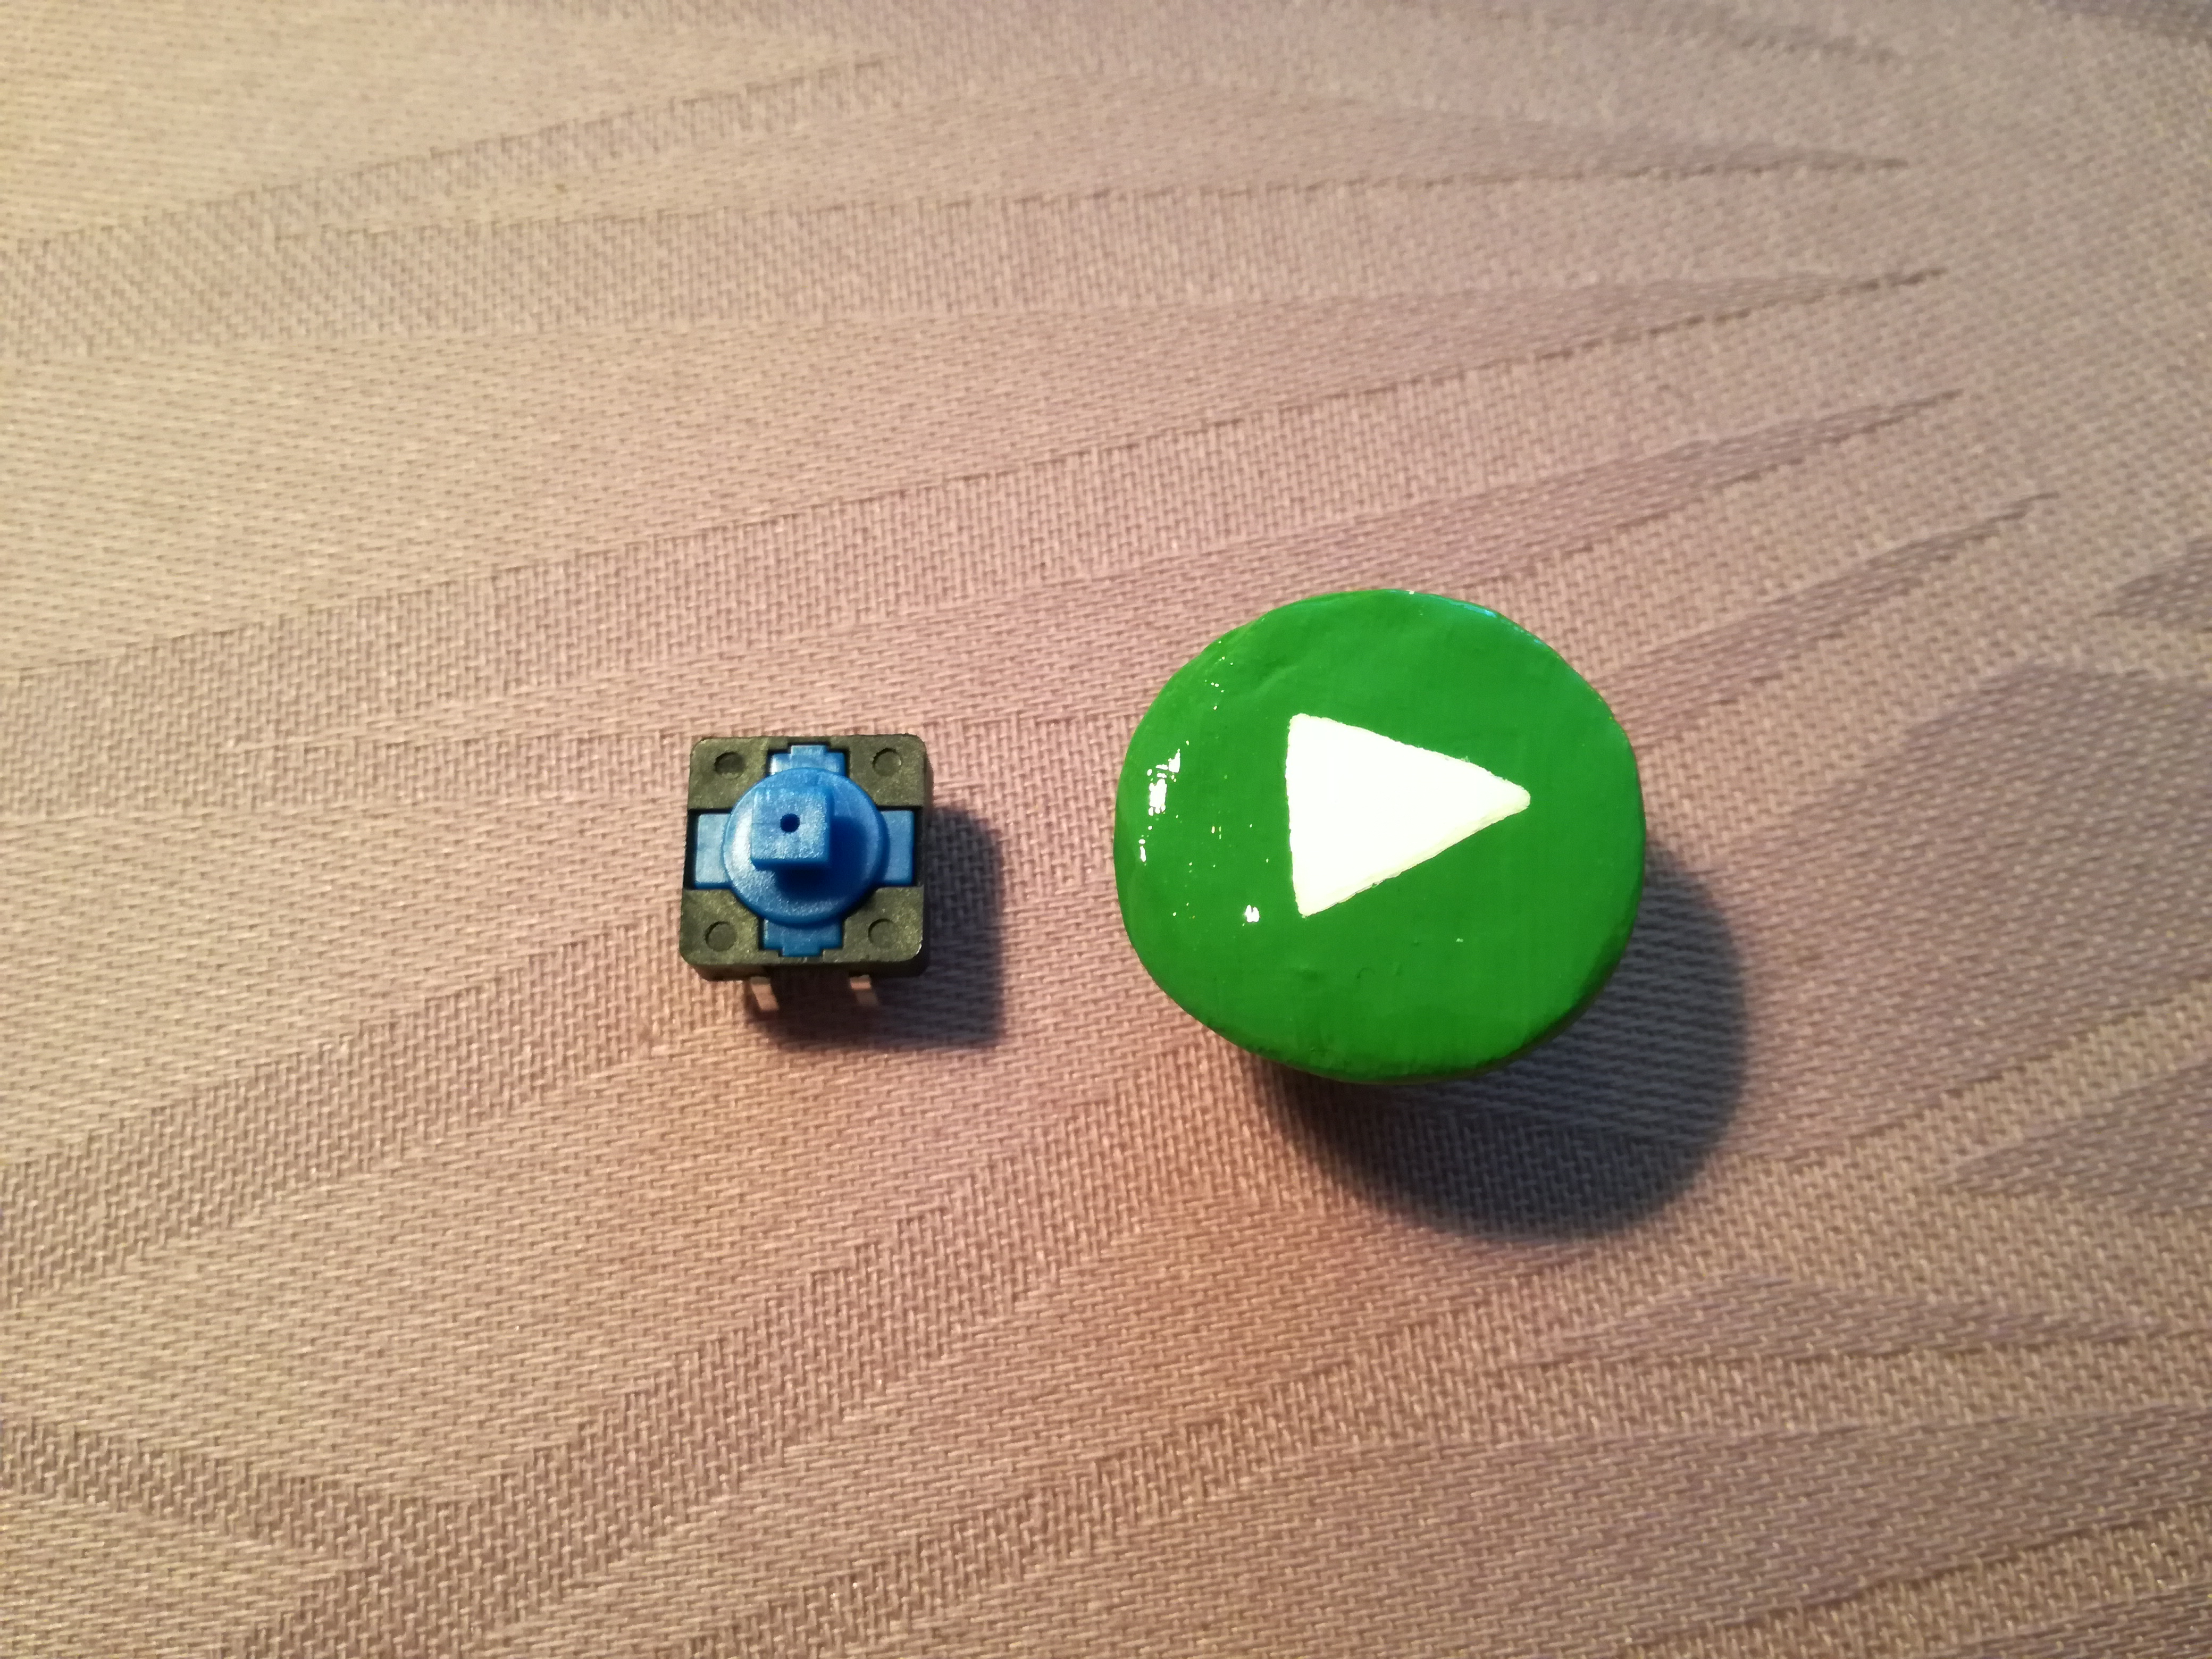
\includegraphics[width=0.7\linewidth]{figure/Design/buttons}
		\caption{The button used, without and with the painted shell. All of the other interface buttons were made in a similar fashion.}
		\label{fig:buttons}
	\end{figure}
		
\section{The mat}\label{sec:theMat}%Daniel
	Before any construction could take place, materials should be chosen. This started out with research and development(R\&D) into pressure sensors, but was quickly diverged from as most could not hold much weight. From here the direction changed to DIY projects that included pressure plates, such as this tutorial to make pressure plates for a haunted house\footnote{\url{http://www.instructables.com/id/Use-a-DIY-Pressure-Plate-Switch-to-Automate-Your-H/}}, which provided the base idea for the fields' construction. The field at this point would not be sturdy enough, to withstand many children jumping around on it for an extended period of time. To make the fields more sturdy and able to persist through many uses, a thin foam layer with holes was inserted in between the top and bottom layer of foil. With that, the final field structure was finished and the result can be seen in \autoref{fig:finalField}.\\
	
	\begin{figure}[H]
		\centering
		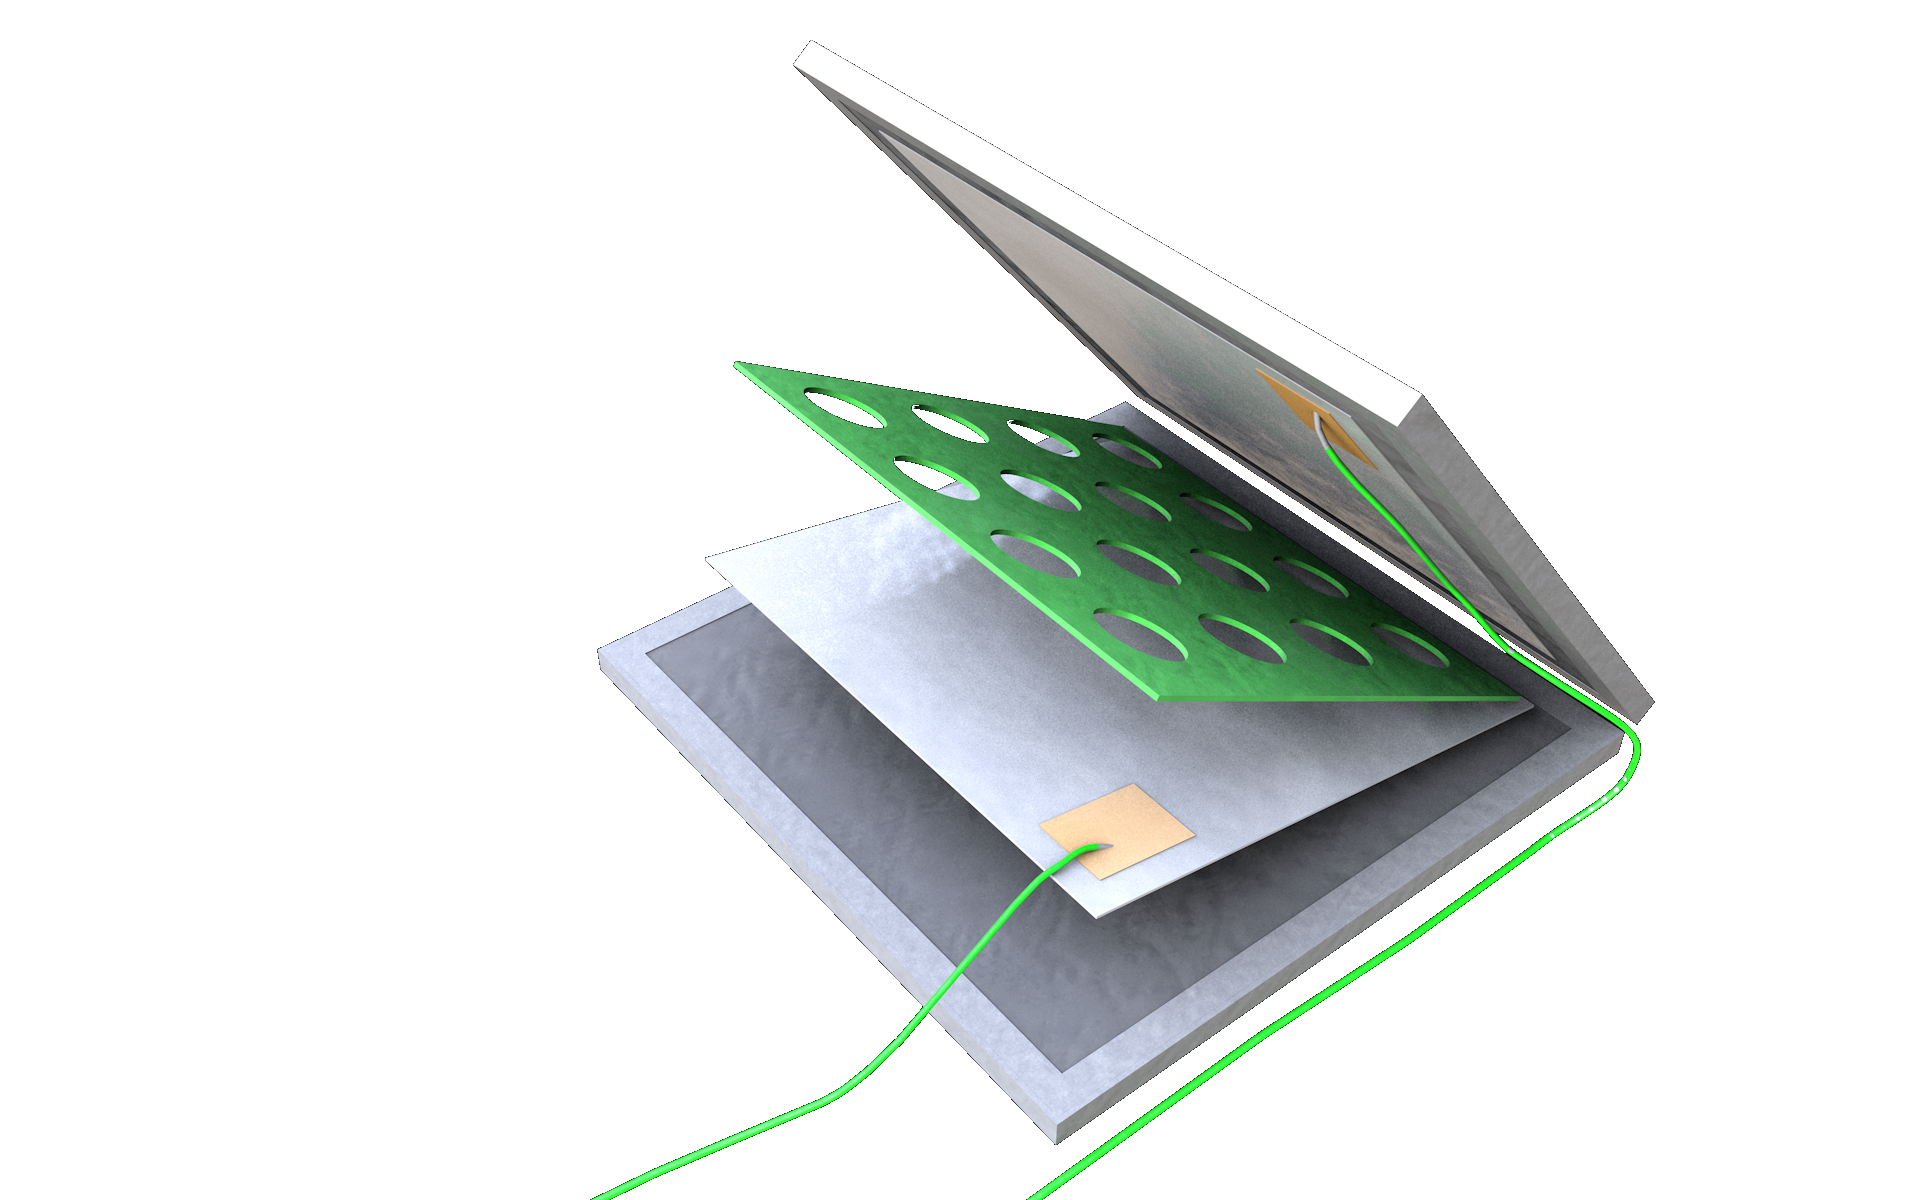
\includegraphics[width=1\linewidth]{figure/Implementation/Medialogyp4mat}
		\caption{The final structure of the mat's fields, with foil on the inside of the top and bottom, and a thin foam layer in the middle, to reinflate the field after it's been activated. The bottom wire is ground, while the top wire is attached to the Arduino Mega.}
		\label{fig:finalField}
	\end{figure}

	After the structure of the fields was settled, twenty identical pieces had to be made, and put together in the 4x5 layout. In between each column of fields, foam tubes were laid down, to funnel the wires through, and to separate the columns. To make the entire mat not fall apart, everything was duct taped together, so the mat stayed as one big piece. The finished mat can be seen in \autoref{fig:finalMat}.
	\begin{figure}[H]
		\centering
		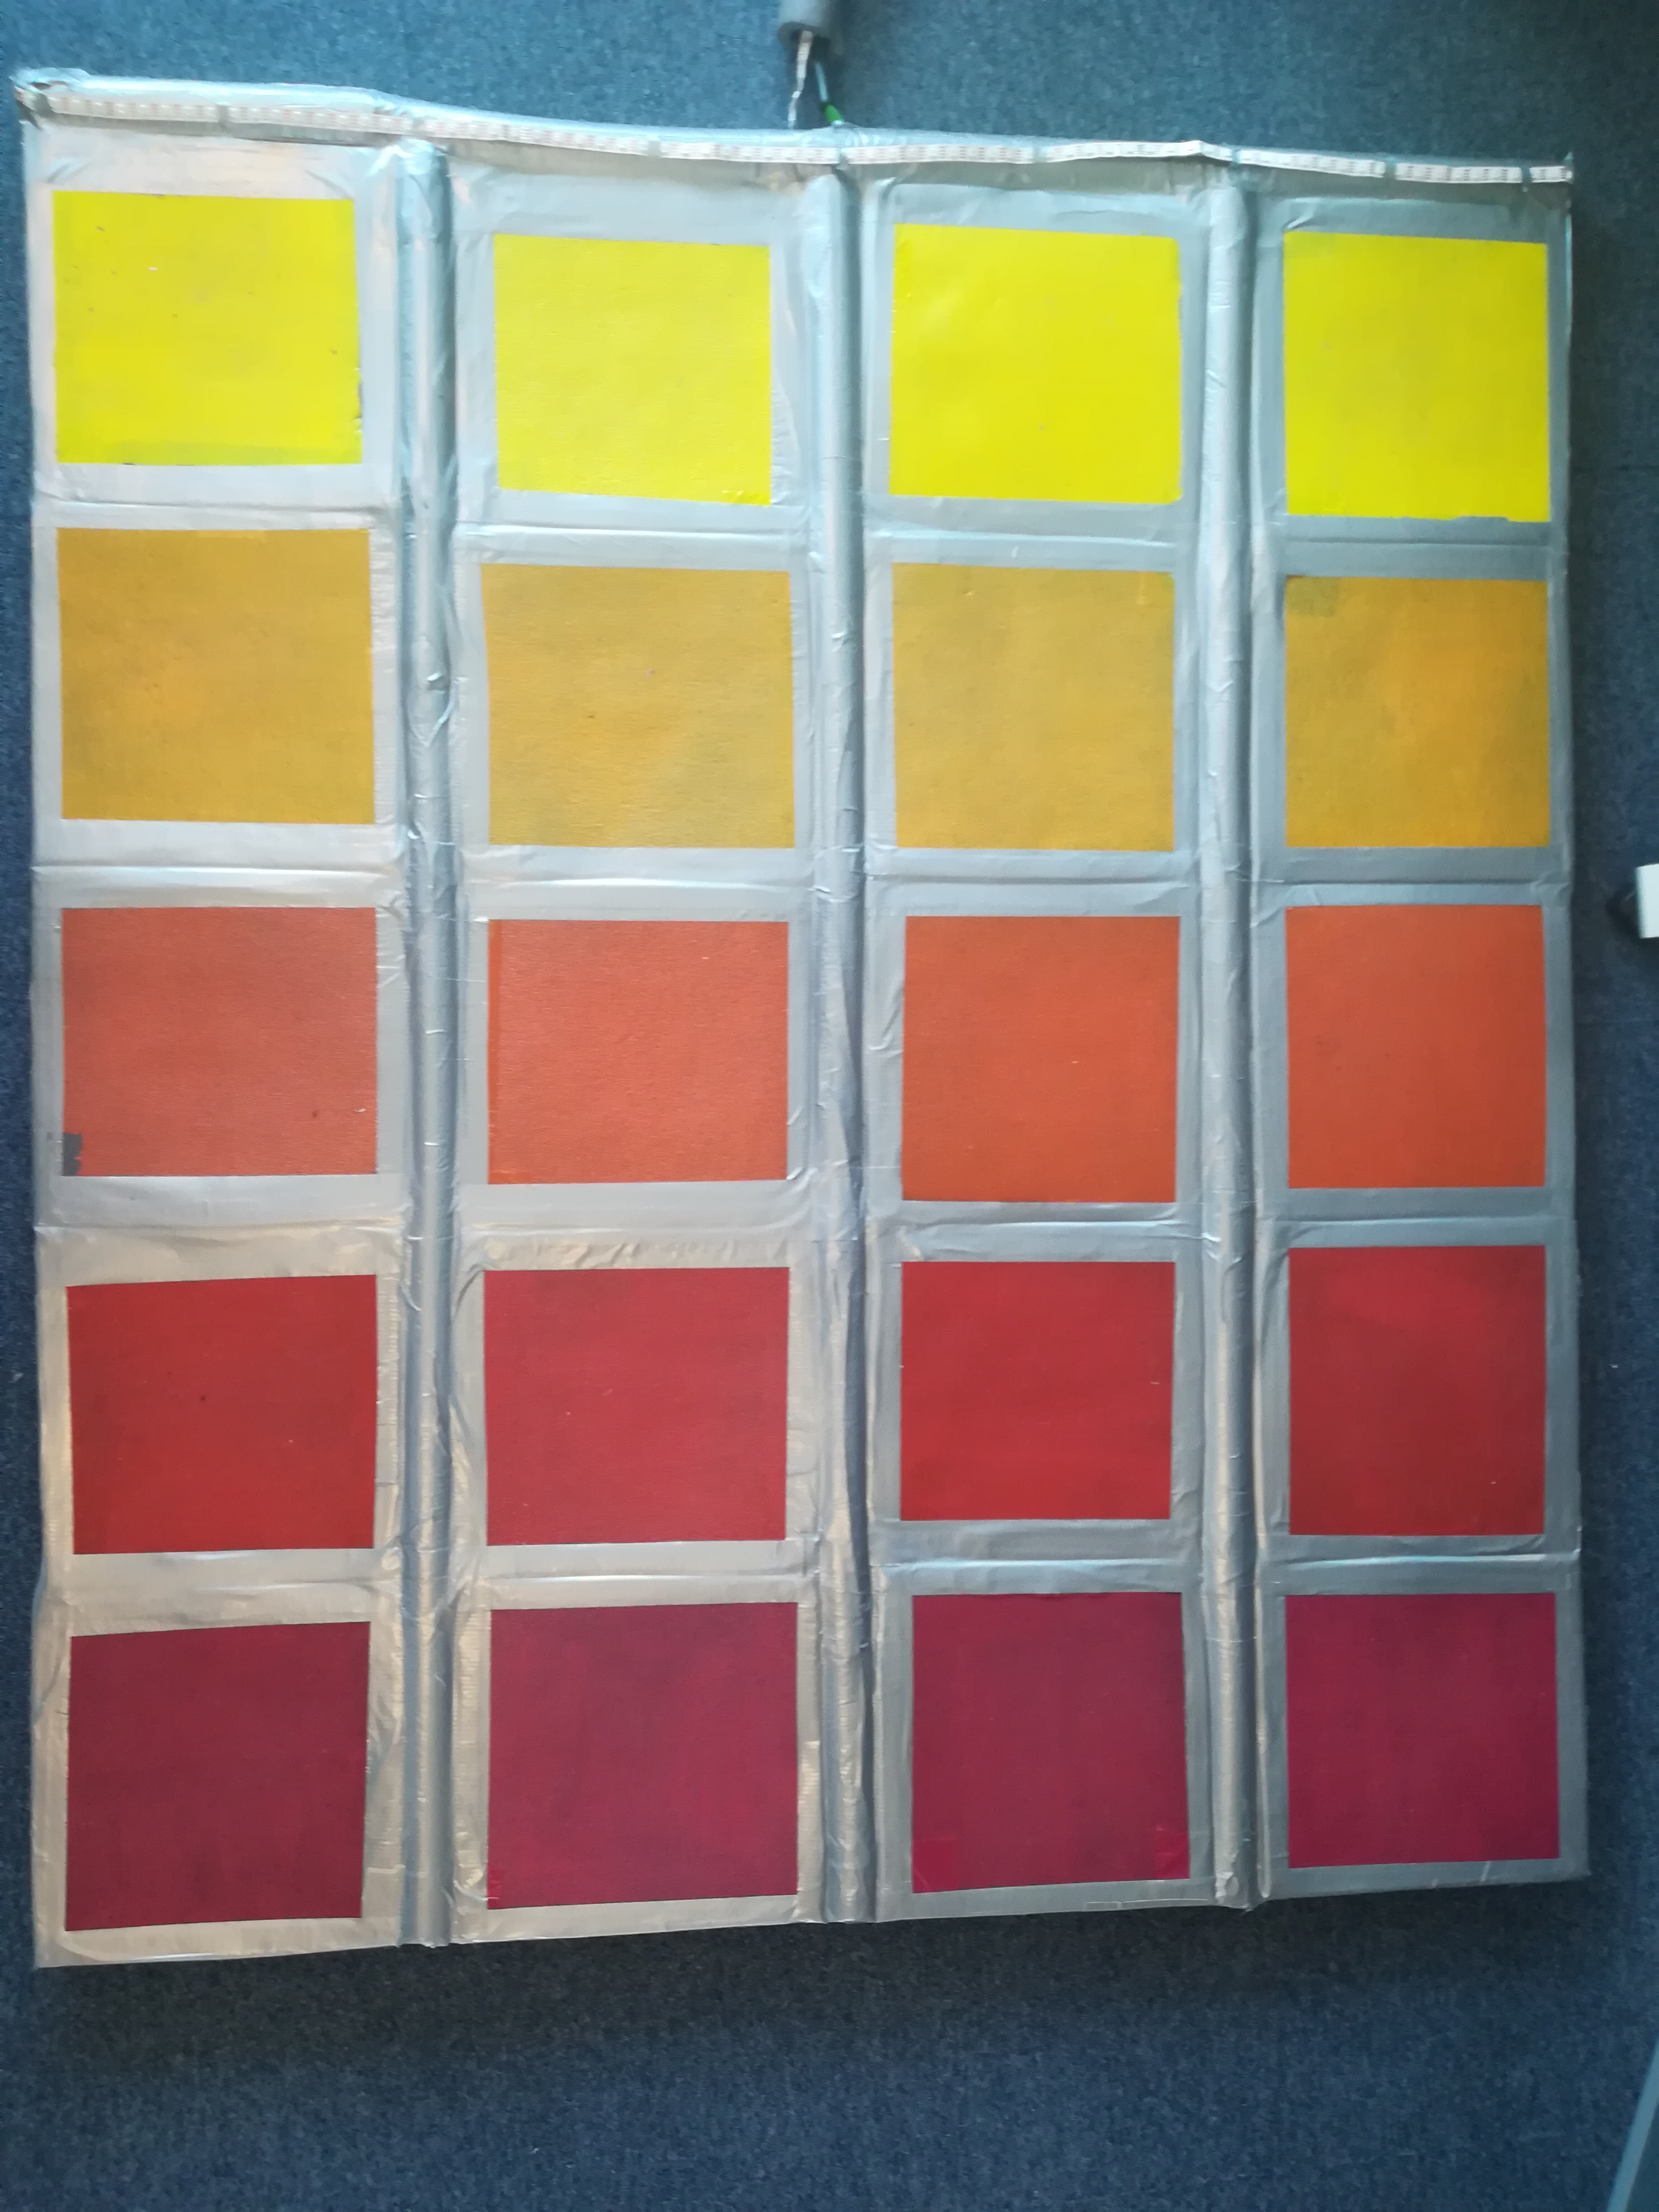
\includegraphics[width=0.42\linewidth]{figure/Implementation/fullMat}
		\caption{The entire mat, duct taped together, and painted with the colour scheme chosen in the design chapter.}
		\label{fig:finalMat}
	\end{figure}
	
 	As explained in \autoref{improvementsUsability}, there was a need for an LED strip to highlight the active beat on the mat. The LED strip that was obtainable and was compatible with the FastLed library was the APA102/SK9822 LED strip akin to this one\footnote{APA102/SK9822 LED strip: \url{http://www.ipixelleds.com/index.php?id=125}}. The strip was duct taped along the top of the mat as seen in \autoref{fig:stripMat}.
 	
 	\begin{figure}[H]
 		\centering
 		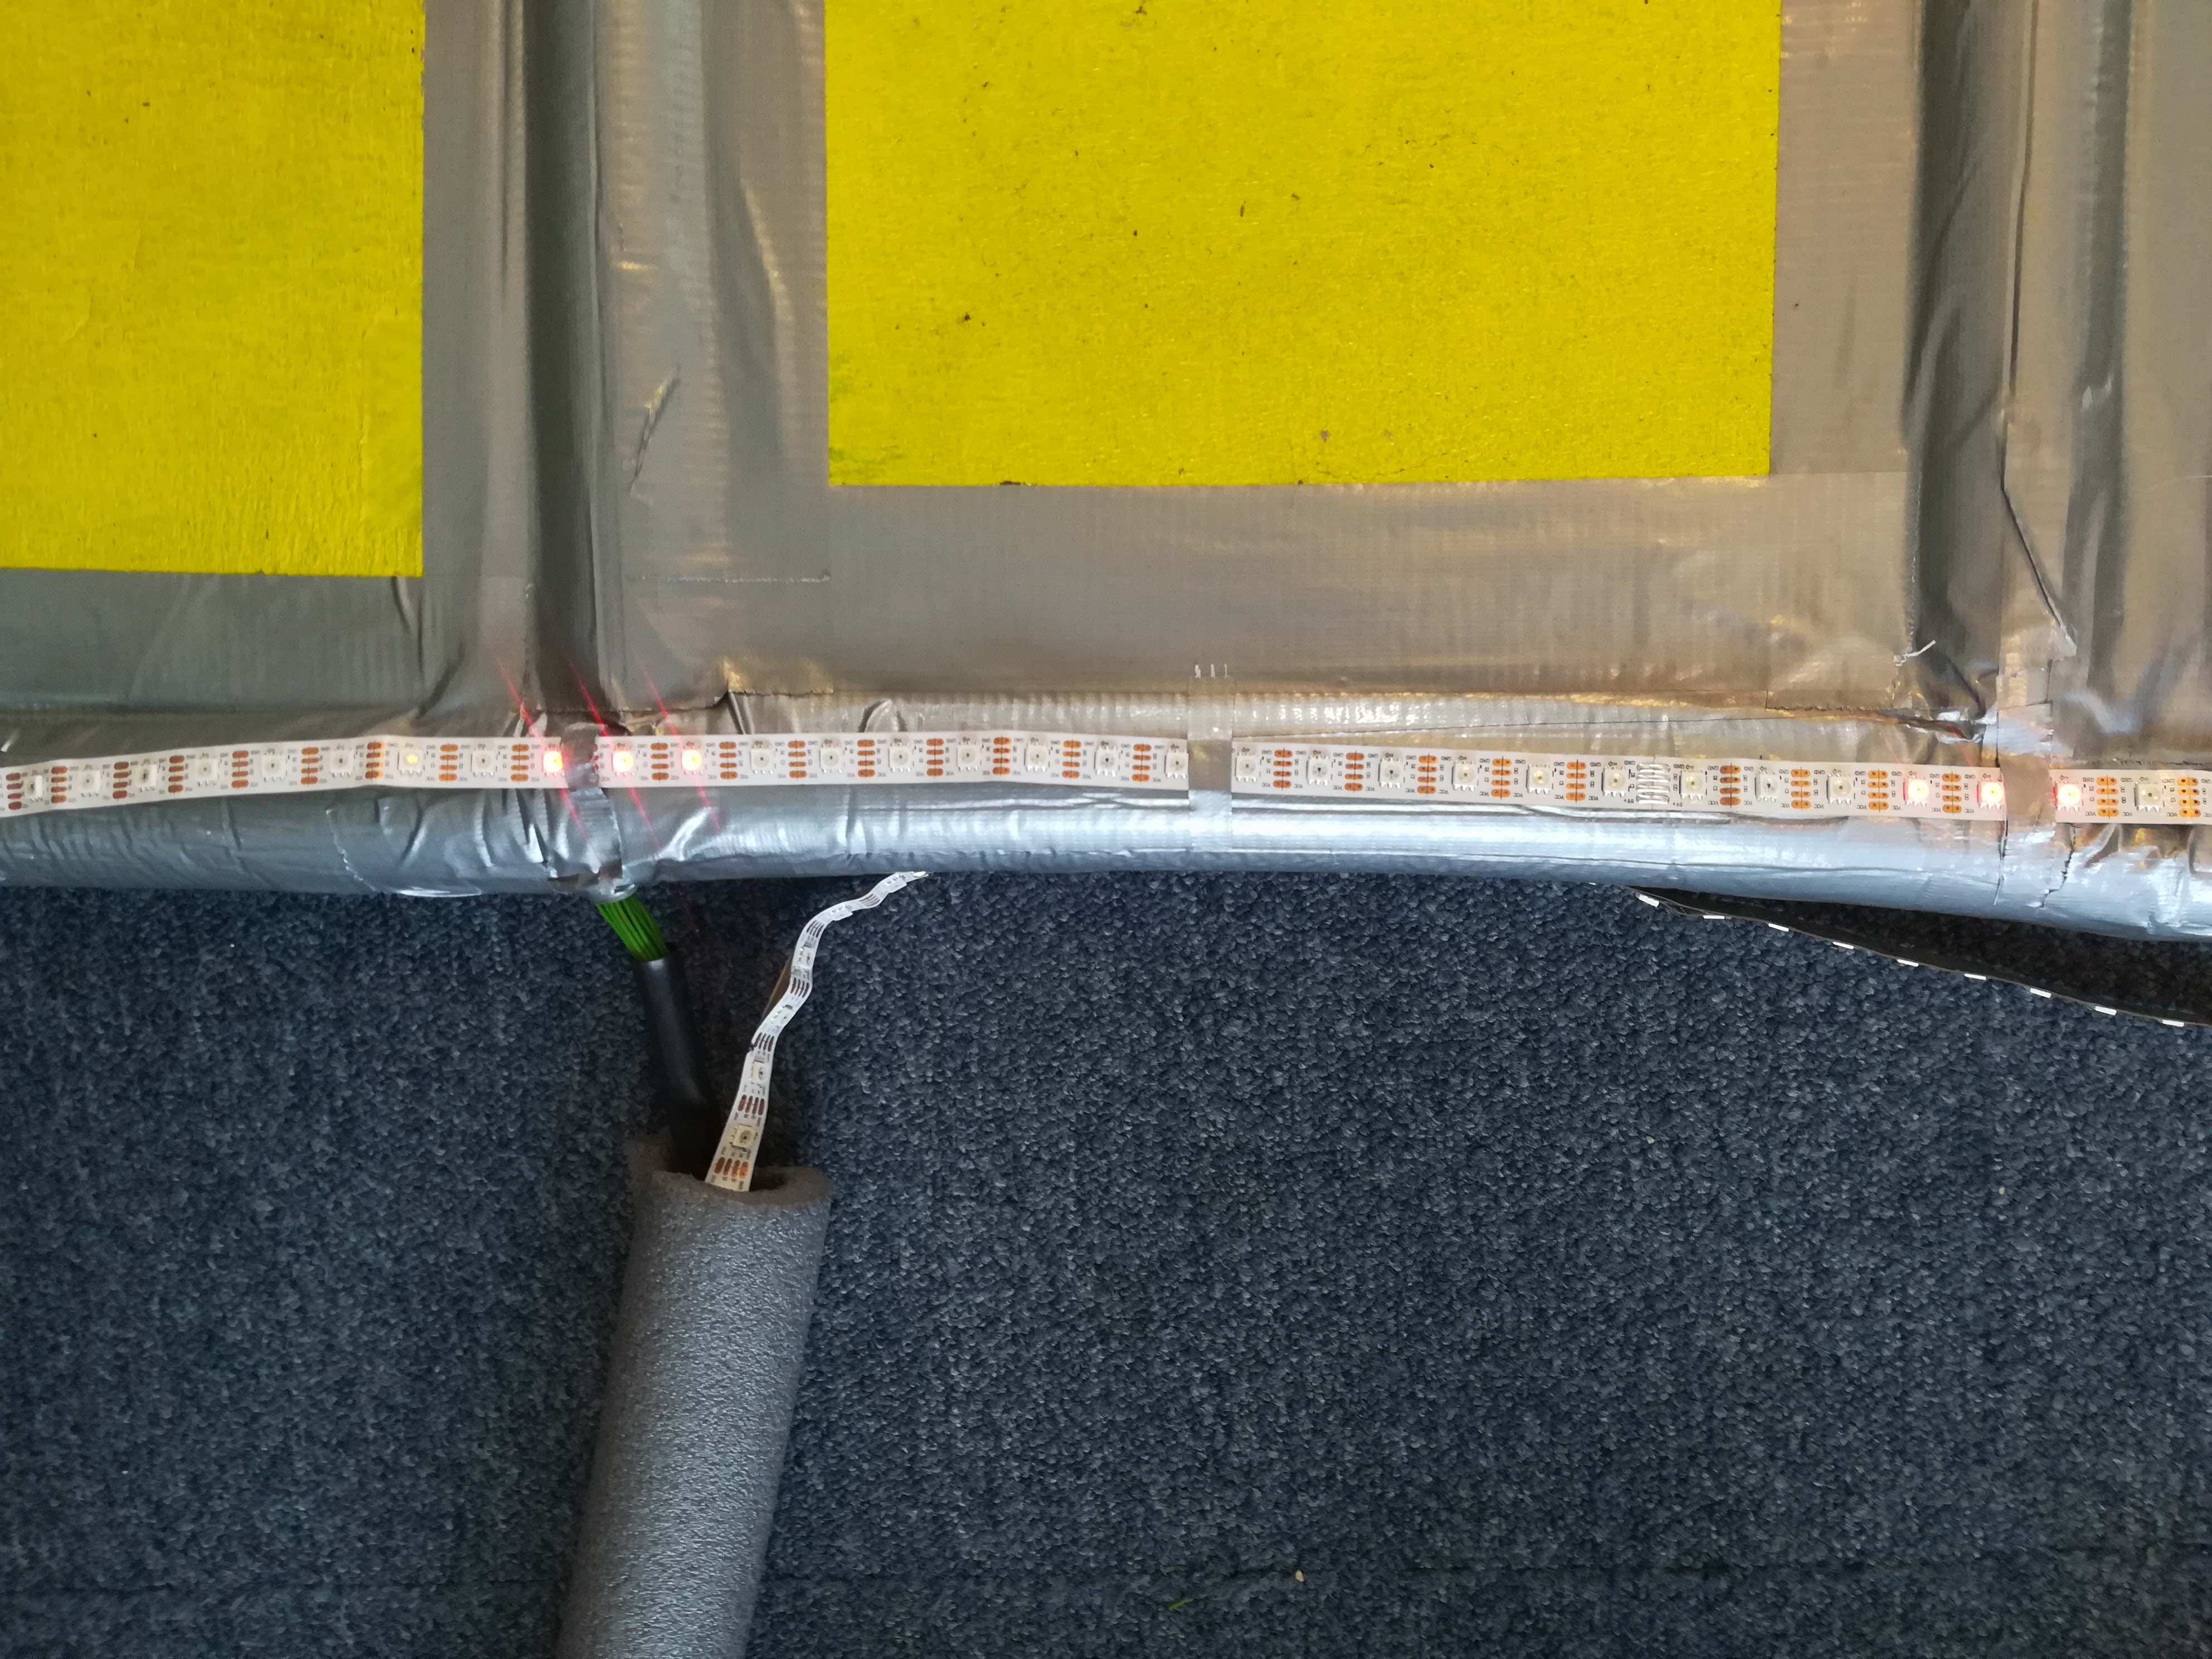
\includegraphics[width=0.8\linewidth]{figure/Implementation/stripMat}
 		\caption{Image of the LED strip that was placed on the top part of the mat to indicate the beats playing.}
 		\label{fig:stripMat}
 	\end{figure}
	
\section{Circuit}
In order to describe the electronics of the system in more detail, a schematic was made (See \autoref{fig:schematic}).
In order to simplify the schematic and save space, only one column(5 fields) of the mat is accounted for. This is highlighted in green in the figure. The remaining columns are repetitions and have been deliberately ignored. The same goes for the buttons on the control box interface, which are all discrete momentary push button switches. Since the sequence buttons also had neighboring LEDs, one of these was included in the schematic. This is highlighted in red.

	\begin{figure}[H]
	\centering
	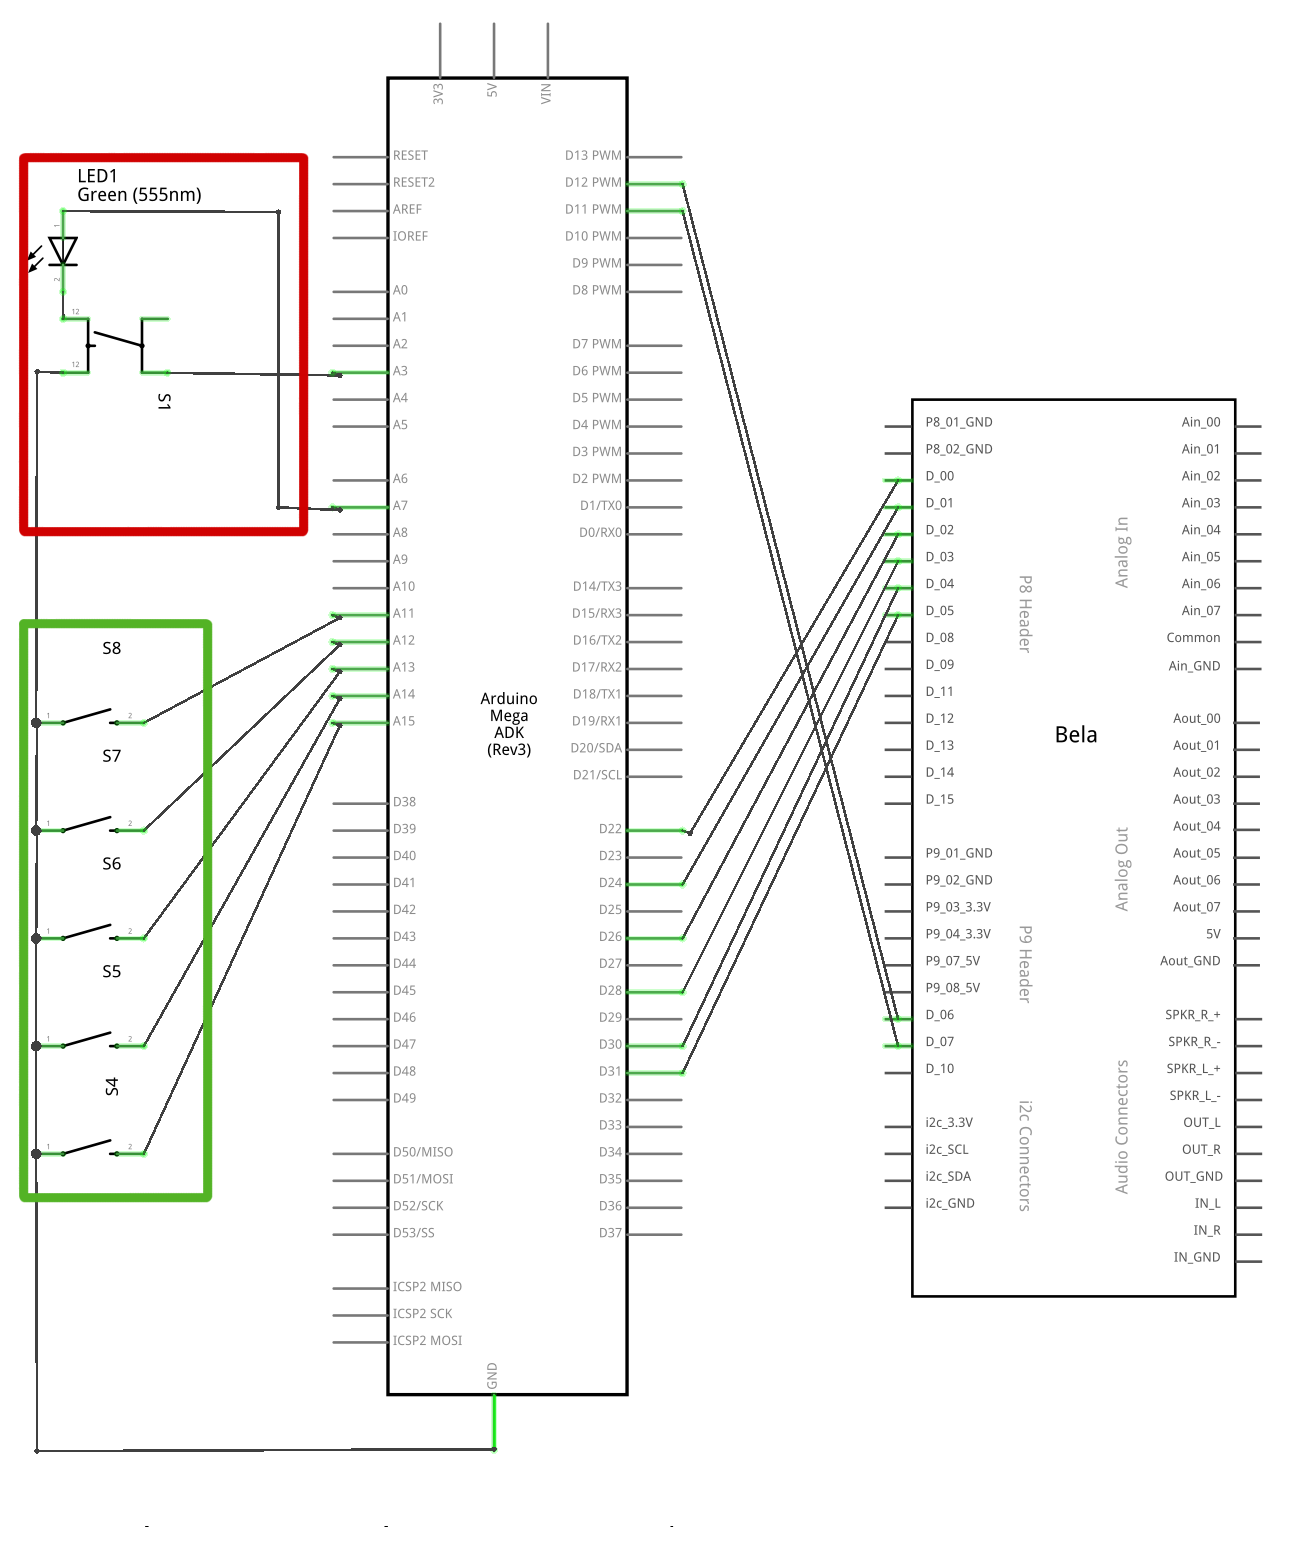
\includegraphics[width=1\linewidth]{figure/Implementation/project_schem_marked.png}
	\caption{Figure showing a simplified schematic of the system. The green square represents one single columns of fields on the mat. The red square represents a single button and LED form the interface on the control box.}
	\label{fig:schematic}
\end{figure}

The figure shows the connection between the Arduino Mega and the Bela. The Arduino sends a signal through 5 pins (D22-D30) to trigger the 5 different tones on the Bela(D\_00-D\_04). When changing the octave the Arduino sends either an up or down signal through pin D12 or D11 respectively to the Bela's allocated octave pins (D\_06 and D\_07). The last connection between the Mega and Bela is a count-in, sound playing on every record or play button press. This is connected from the Arduinos D31 to the Bela's D\_05.